% ==========================================
% SEÇÃO 4: TECNOLOGIAS DE TELAS E DISPLAYS
% ==========================================
\section{Tecnologias de Displays}

% --- SLIDE 1: IPS ---
\begin{frame}{Telas IPS: Alinhamento de Cristais e Precisão Cromática}
    \begin{columns}[T]
        \begin{column}{0.55\textwidth}
            \small
            \begin{itemize}
                \item \textbf{Orientação em Plano (In-Plane):} Os cristais líquidos giram paralelamente ao plano do painel quando submetidos a um campo elétrico.
                \vspace{0.2cm}
                \item \textbf{Ângulo de Visão Estendido:} Consistência de cor e contraste mesmo em observações oblíquas periféricas (até 178°).
                \vspace{0.2cm}
                \item \textbf{Fidelidade Cromática:} Modelo padrão para calibração profissional em design gráfico, engenharia de interface e fotografia.
            \end{itemize}
        \end{column}
        
        \begin{column}{0.45\textwidth}
            \begin{figure}
                \centering
                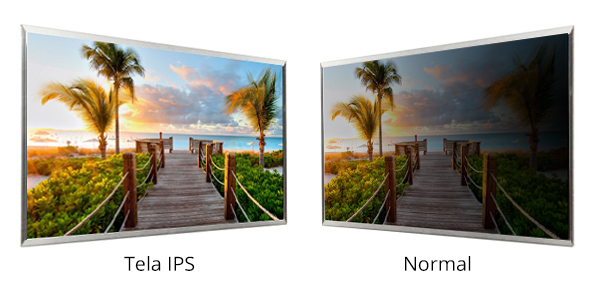
\includegraphics[width=0.9\textwidth]{images/ips.png}
                \caption{Mecanismo de rotação paralela dos cristais IPS.}
            \end{figure}
        \end{column}
    \end{columns}

    \note{
        \footnotesize
        \begin{columns}[T]
            \begin{column}{0.49\textwidth}
                \textbf{Física Óptica do Painel:}
                \begin{itemize}
                    \setlength{\itemsep}{1pt}
                    \item \textbf{Bloqueio de Luz:} Como os cristais apenas barram a luz polarizada de um backlight sempre ativo, o fechamento físico dos canais não é perfeito.
                    \item \textbf{Contraste Nativo Baixo:} Painéis IPS convencionais raramente ultrapassam a razão estática de 1000:1, fazendo com que tons pretos pareçam cinza escuro em ambientes de baixa iluminação.
                \end{itemize}
            \end{column}

            \begin{column}{0.49\textwidth}    
                \textbf{Limitações de Hardware:}
                \begin{itemize}
                    \setlength{\itemsep}{1pt}
                    \item \textbf{Backlight Bleeding:} Defeito estrutural ou pressão mecânica excessiva na carcaça que permite o escape de luz pelas bordas físicas da tela.
                    \item \textbf{IPS Glow:} Fenômeno óptico difuso onde o brilho do fundo parece flutuar dependendo do ângulo de visão, muito visível nos cantos de displays grandes a distâncias curtas.
                \end{itemize}
            \end{column}
        \end{columns}
    }
\end{frame}

% --- SLIDE 2: MINI-LED ---
\begin{frame}{Telas Mini-LED: Evolução do Backlight e Alto Brilho}
    \begin{columns}[T]
        \begin{column}{0.55\textwidth}
            \small
            \begin{itemize}
                \item \textbf{Retroiluminação Avançada:} Substitui as lâmpadas de borda tradicionais por milhares de diodos minúsculos dispostos atrás da matriz LCD.
                \vspace{0.2cm}
                \item \textbf{Atenuação Local (FALD):} Agrupamento dos LEDs em centenas ou milhares de zonas controladas independentemente por software.
                \vspace{0.2cm}
                \item \textbf{Pico de Luminância:} Excelente capacidade para HDR agressivo, alcançando níveis de brilho muito superiores ao OLED comercial.
            \end{itemize}
        \end{column}
        
        \begin{column}{0.45\textwidth}
            \begin{figure}
                \centering
                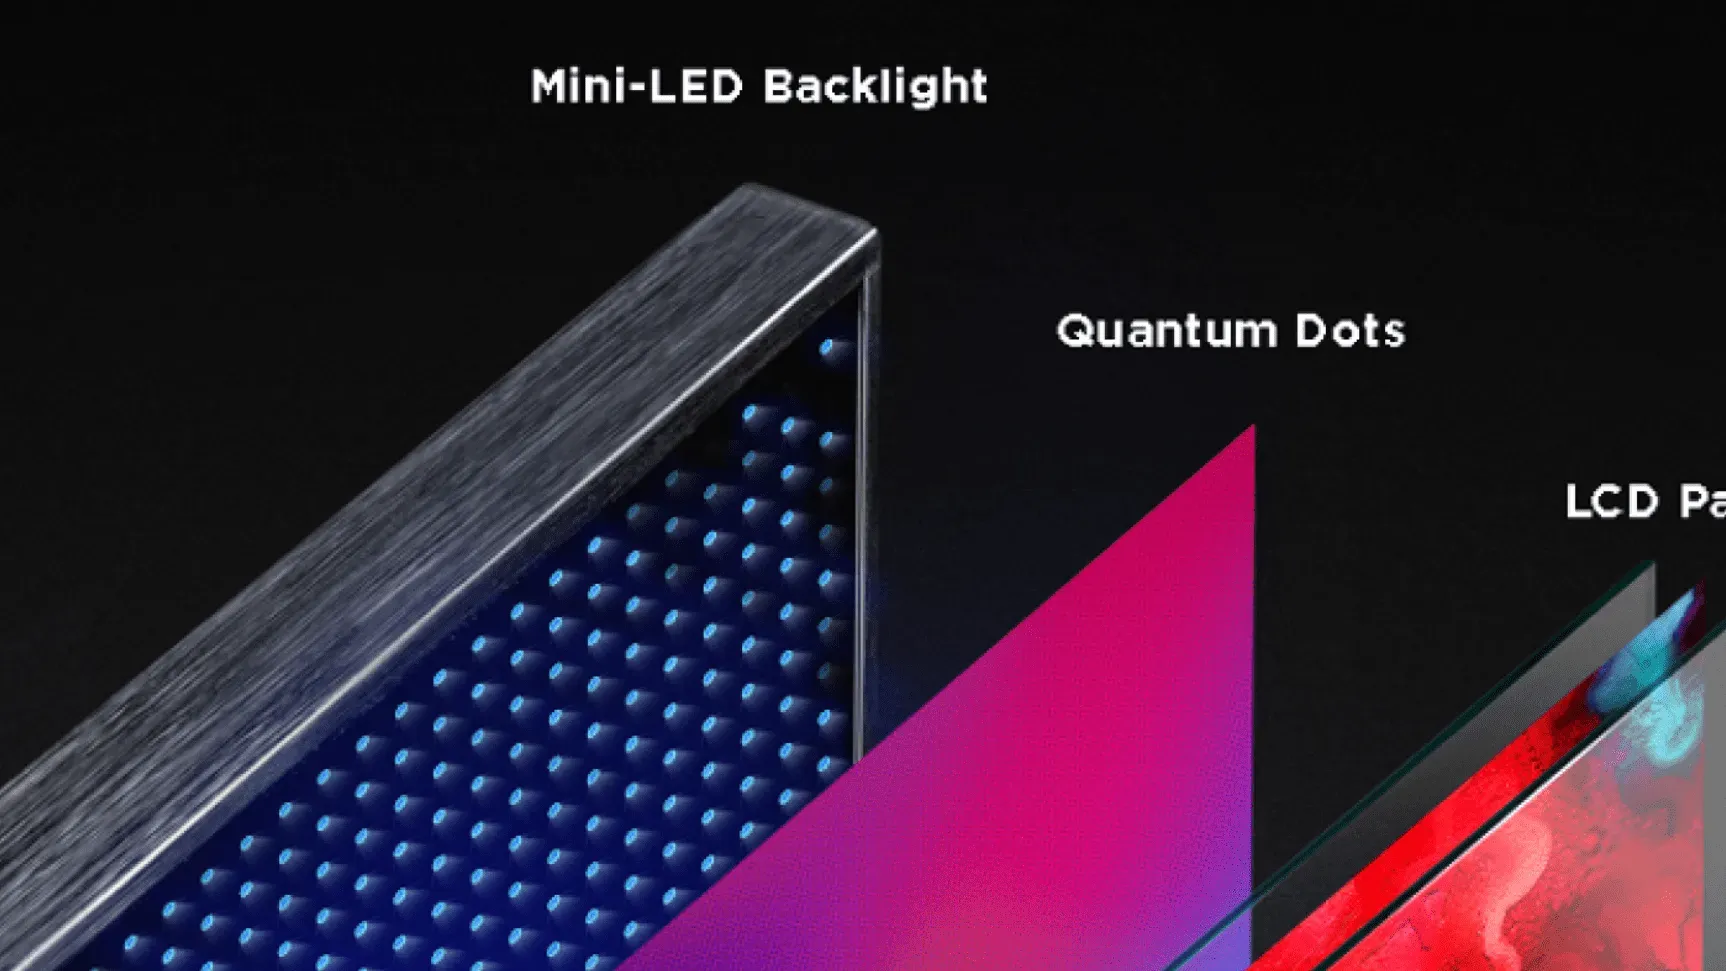
\includegraphics[width=0.9\textwidth]{images/min_led.png}
                \caption{Zonas de retroiluminação em matriz Mini-LED.}
            \end{figure}
        \end{column}
    \end{columns}

    \note{
        \footnotesize
        \begin{columns}[T]
            \begin{column}{0.49\textwidth}
                \textbf{Engenharia de Iluminação:}
                \begin{itemize}
                    \setlength{\itemsep}{1pt}
                    \item \textbf{Mecanismo:} Une a durabilidade e estabilidade química dos compostos inorgânicos (sem risco de burn-in) à modulação espacial de contraste.
                    \item \textbf{O Efeito Blooming:} Limitação física decorrente do desalinhamento de resolução entre a matriz de LEDs (zonas) e a matriz de subpixels LCD. Objetos brilhantes pequenos em fundos pretos geram um "halo" ou vazamento de luz indesejado.
                \end{itemize}
            \end{column}

            \begin{column}{0.49\textwidth}    
                \textbf{Algoritmos de Controle:}
                \begin{itemize}
                    \setlength{\itemsep}{1pt}
                    \item \textbf{Latência de Shaders:} O driver de hardware precisa analisar o frame de entrada e calcular o mapa de atenuação para as zonas de iluminação em tempo real. Algoritmos mal otimizados geram atraso perceptível na mudança de brilho (\textit{luminance lag}).
                \end{itemize}
            \end{column}
        \end{columns}
    }
\end{frame}

% --- SLIDE 3: OLED ---
\begin{frame}{Telas OLED: Emissão Direta e Contraste Absoluto}
    \begin{columns}[T]
        \begin{column}{0.55\textwidth}
            \small
            \begin{itemize}
                \item \textbf{Matriz Autoemissiva:} Cada pixel é composto por diodos orgânicos que emitem sua própria luz sob corrente elétrica.
                \vspace{0.2cm}
                \item \textbf{Contraste Infinito:} A representação do preto digital ($0,0,0$) desliga o emissor por completo.
                \vspace{0.2cm}
                \item \textbf{Tempo de Resposta:} Transição de estado quase instantânea (sub-milissegundo), eliminando rastros visíveis (\textit{ghosting}).
            \end{itemize}
        \end{column}
        
        \begin{column}{0.45\textwidth}
            \begin{figure}
                \centering
                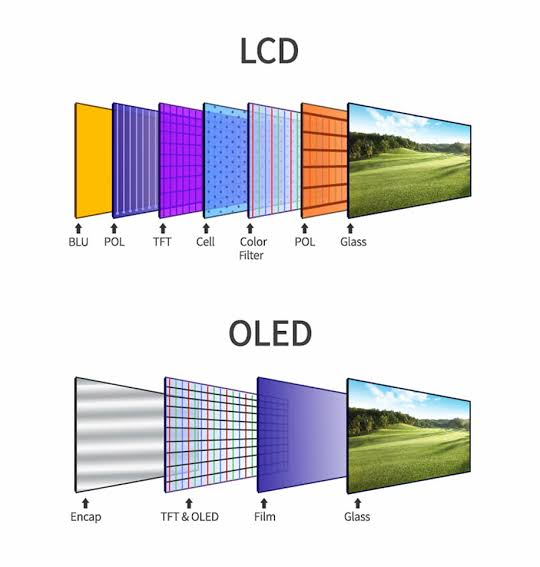
\includegraphics[width=0.9\textwidth]{images/oled.png}
                \caption{Funcionamento de subpixels autoemissivos OLED.}
            \end{figure}
        \end{column}
    \end{columns}

    \note{
        \footnotesize
        \begin{columns}[T]
            \begin{column}{0.49\textwidth}
                \textbf{Física do Estado Sólido:}
                \begin{itemize}
                    \setlength{\itemsep}{1pt}
                    \item \textbf{Arquitetura:} Elimina a necessidade de uma camada difusora e de um backlight centralizado, reduzindo drasticamente a espessura do painel.
                    \item \textbf{O Problema do Burn-in:} Degradação fotoquímica diferencial dos materiais orgânicos. O subpixel azul possui menor eficiência e exige maior corrente, acelerando seu desgaste sob imagens estáticas.
                \end{itemize}
            \end{column}

            \begin{column}{0.49\textwidth}    
                \textbf{Controle de Baixo Nível:}
                \begin{itemize}
                    \setlength{\itemsep}{1pt}
                    \item \textbf{Modulação de Brilho:} Telas OLED frequentemente utilizam PWM (Modulação por Largura de Pulso) para controlar o brilho, o que pode causar cintilação perceptível (\textit{flicker}) e fadiga ocular em frequências baixas.
                    \item \textbf{Eficiência Energética:} O consumo é dinâmico e diretamente proporcional à luminância média da imagem (APL - \textit{Average Picture Level}), tornando o \textit{Dark Mode} uma otimização de hardware real.
                \end{itemize}
            \end{column}
        \end{columns}
    }
\end{frame}